\documentclass[paper=a4, fontsize=11pt]{article} 

\usepackage[T1]{fontenc} 

\usepackage[utf8]{inputenc}
\usepackage[francais]{babel} 
\usepackage{mathtools}
\usepackage{amssymb}
\usepackage{alltt}
\usepackage{float}
\usepackage{graphicx}
\usepackage[colorinlistoftodos]{todonotes}
\usepackage{geometry}
\usepackage{hyperref}
\usepackage{enumitem}
\usepackage{subcaption}
\usepackage[ruled,vlined]{algorithm2e}

\newcommand{\argmin}[1]{\underset{#1}{\operatorname{argmin}}\;}

\title{\normalfont \normalsize 
\huge Pointing error correction}

\author{Jules Kozolinsky, Vincent Matthys}

\date{}

\begin{document}
\maketitle

\section{Attitude of a Satellite}

\begin{figure}[h]
	\centering
	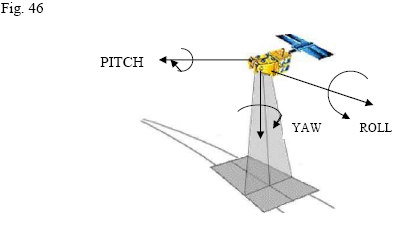
\includegraphics[width=0.5\textwidth]{figures/angles.jpg}
   \caption{ Roll, pitch and yaw angles.}
   \label{angles}
\end{figure}

\section{Satellite attitude error effects on stereo images}
\label{sec:sensibility}

\section{Correction of Relative Pointing Error}
\cite{de2014automatic}\\

A simple way to correct the relative pointing error is thus to transform one of the two images, in such a way that the corresponding points fall on the respective epipolar curves: given two images $u$, $v$ and a set of correspondences $(\textbf{x}_i , \textbf{x}'_i)_{i=1...N}$ , we search for a translation $f$ such that, for all $i$, the transformed point $f(\textbf{x}'_i)$ lies on the epipolar curve $epi^{\textbf{x}_i}_{u v}(R)$.
The desired transformation $f^{*}$ minimises the relative pointing error defined by:
\begin{align}
\label{minif}
f^* = \argmin{f} \dfrac{1}{N} \sum\limits_{i=1}^{N} d(f(\textbf{x}'_i), epi^{\textbf{x}_i}_{u v}(R))
\end{align}

From  \cite{de2014automatic}, we know that the epipolar curve $epi^{\textbf{x}_i}_{u v}(R)$ is approximated up to $0.05$ pixels by the straight line $F\textbf{x}_i$, where $F$ is
the affine fundamental matrix between the two views for the considered tile. As this fundamental matrix is an \textit{affine} fundamental matrix, all the lines $F\textbf{x}_i$ are parallel. 

\subsection{Roll and Pitch Angles}
Because of sensitivity issues, we can take only roll and pitch error into account. Therefore according to section \ref{sec:sensibility}, we search for a transformation $f$ such that
\begin{align*}
f(\textbf{x}) = T\textbf{x}
\end{align*}
where $T$ is a translation:
\begin{align*}
T = 
\begin{pmatrix} 
1 & 0 & t_1 \\
0 & 1 & t_2 \\
0 & 0 & 1
\end{pmatrix}
\end{align*}
So we have, for $ \textbf{x} = (  x \; y \; 1)^T $, 
\begin{align*}
f(\textbf{x}) = T\textbf{x} = 
\begin{pmatrix} 
x + t_1 \\
y + t_2 \\
1
\end{pmatrix}
\end{align*}

\subsubsection{Pointing error after rectification}
Without any additional restriction, we may assume that these lines are horizontal (otherwise just do a change of coordinates). The horizontal line $F\textbf{x}_i$ can be written, in homogeneous coordinates, as
\begin{align*}
F\textbf{x}_i = \left[ 0 \; 1 \; c_i \right]
\end{align*}
With these notations, for each point correspondence $(\textbf{x}_i , \textbf{x}'_i)$, we have
\begin{align*}
e(\textbf{x}_i, \textbf{x}'_i) = d(\textbf{x}'_i, epi^{\textbf{x}_i}_{u v}(R)) = d(\textbf{x}'_i, F\textbf{x}_i) = | y'_i + c_i|
\end{align*}

Here the error $e$ is invariant to any horizontal translation, thus the search for a translation minimizing the relative pointing error of formula (\ref{minif}) can be restricted to vertical translations only. With a vertical translation of parameter $t$, the error becomes
\begin{align*}
E(T) = \dfrac{1}{N} \sum\limits_{i=1}^{N} d(T\textbf{x}'_i, F\textbf{x}_i) = \dfrac{1}{N} \sum\limits_{i=1}^{N} | y'_i + t+ c_i|
\end{align*}
The translation that minimizes this sum is given by the geometric median (Weiszfeld, 1937) of the vector $(-y'_i - c_i )_{i=1...N}$.  The relative pointing error can thus be minimized in a tile by applying a translation to one of the images. Note that the median is robust against outliers, thus this correction procedure works well even in the presence of false matches.

\subsubsection{Pointing before after rectification}
In the general case, we have:
\begin{align*}
F\textbf{x}_i = \left( a_i \; b_i \; c_i \right)^T
\end{align*}
With these notations, the error to minimize is then:
\begin{align*}
E(T) &= \dfrac{1}{N} \sum\limits_{i=1}^{N} d(T\textbf{x}'_i, F\textbf{x}_i) = \dfrac{1}{N} \sum\limits_{i=1}^{N} \dfrac{|a_i(x'_i + t_1) + b_i(y'_i +t_2)+ c_i|}{\sqrt{a_i^2 + b_i^2}}
\end{align*}\\
As this fundamental matrix is an \textit{affine} fundamental matrix, all the lines $F\textbf{x}_i$ are parallel, \textit{i.e.} 
\begin{align*}
F\textbf{x}_i = \left( a\; b\; c_i \right)^T
\end{align*}\\
We can then write the error as :
\begin{align*}
E(t_1, t_2) = \dfrac{1}{N\sqrt{a^2 + b^2}} \sum\limits_{i=1}^{N} |ax'_i+ by'_i + c_i + at_1 + bt_2|
\end{align*}
$=\underset{y \in \mathbb{R}^n}{\operatorname{arg\,min}} \sum_{i=1}^N \left \| z_i-y \right \|_2$\\
$y = 
\begin{pmatrix} 
- at_1 \\
- bt_2 \\
0
\end{pmatrix}
$
$z_i = 
\begin{pmatrix} 
ax'_i \\
by'_i \\
c_i
\end{pmatrix}$
%\paragraph{Compute vectors $p$\\}
%We can compute the vectors going from the projection of $\textbf{x}'_i$ on $F\textbf{x}_i$ to $\textbf{x}_i$:
%\begin{align*}
%p(\textbf{x}_i, \textbf{x}'_i) &= d(\textbf{x}'_i, F\textbf{x}_i)\dfrac{1}{\sqrt{a_i^2 + b_i^2}}
%\begin{pmatrix} 
%a_i \\
%b_i 
%\end{pmatrix}  \\
%&=
%\dfrac{|a_ix'_i + b_iy'_i + c_i|}{a_i^2 + b_i^2}
%\begin{pmatrix} 
%a_i \\
%b_i \\
%\end{pmatrix}
%\end{align*}

%And we have : 

%\begin{align*}
%\begin{pmatrix} 
%t_1^* \\
%t_2^* \\
%\end{pmatrix} = -\text{median}\left[ p(\textbf{x}_i, \textbf{x}'_i)_{1 \leq i \leq N} \right]
%\end{align*}



\subsection{Roll, Pitch and Yaw Angles}
If we assume that the scene is located at infinity with respect to the satellite, an error in the sensor attitude measurement can be modeled in image space as a translation composed with a rotation. Therefore we have
\begin{align*}
f(\textbf{x}) = MT\textbf{x}
\end{align*}
where $M$ is a rigid transformation and $T$ a translation:\\
\begin{align*} 
M = 
\begin{pmatrix} 
\cos(\theta) & -\sin(\theta) & t_x \\
\sin(\theta) & \cos(\theta) & t_y \\
0 & 0 & 1
\end{pmatrix}, \; 
T = 
\begin{pmatrix} 
1 & 0 & t_1 \\
0 & 1 & t_2 \\
0 & 0 & 1
\end{pmatrix}
\end{align*}
So we have, for $ \textbf{x} = (  x \; y \; 1)^T $, 
\begin{align*}
f(\textbf{x}) = MT\textbf{x} &= 
\begin{pmatrix} 
\cos(\theta) & -\sin(\theta) & t_1\cos(\theta) - t_2\sin(\theta) + t_x \\
\sin(\theta) & \cos(\theta) & t_1\sin(\theta) + t_2\cos(\theta) + t_y \\
0 & 0 & 1
\end{pmatrix} \textbf{x}  \\
&= 
\begin{pmatrix} 
\cos(\theta)x -\sin(\theta)y + t_1\cos(\theta) - t_2\sin(\theta) + t_x \\
\sin(\theta)x + \cos(\theta)y + t_1\sin(\theta) + t_2\cos(\theta) + t_y \\
1
\end{pmatrix}
\end{align*}


\bibliographystyle{plain}
\bibliography{biblio}
\end{document}

